% =====================================================================
%  chunks/ch02b.tex —— 原书 p.23–31（PDF 30–38）
%  第 2 章 §3 收尾（局部平凡纤维化/纤维丛）；§4 同伦群与纤维化. 正合列. 例子（前半）
%  块首续写 p.22 末句「…其」，不写节标题；§4 标题在原书 p.23 页面上，此处写 \section。
% =====================================================================
% [原文 p.23]
完全原像 $p^{-1}(U)\subset X$ 通过一个与投影 $p$「相容」的同胚 $q:p^{-1}(U)\to U\times F$ 同胚于直积 $U\times F$。（这里纤维 $F$ 不必像覆叠空间那样离散。）设 $\{U_\alpha\}$ 是由这样的开集 $U_\alpha$ 组成的 $Y$ 的一个覆盖。于是给定覆盖中任意两个集合 $U_\alpha,U_\beta$，在它们之交 $U_\alpha\cap U_\beta=U_{\alpha,\beta}$ 的完全原像上有两个同胚：
\[
  \phi_\alpha:p^{-1}(U_{\alpha,\beta})\to U_{\alpha,\beta}\times F,
\]
\[
  \phi_\beta:p^{-1}(U_{\alpha,\beta})\to U_{\alpha,\beta}\times F.
\]
映射 $\lambda_{\alpha,\beta}=\phi_\alpha\circ\phi_\beta^{-1}:U_{\alpha,\beta}\times F\to U_{\alpha,\beta}\times F$ 保持纤维，并在底空间 $U_{\alpha,\beta}$ 上诱导恒等映射。因此它具有如下形式
\[
  \lambda_{\alpha,\beta}(w,f)=\bigl(w,\hat\lambda_{\alpha,\beta}(w)(f)\bigr),
\]
其中 $\hat\lambda_{\alpha,\beta}(w):F\to F$ 是 $w$ 上方纤维的同胚，并且连续依赖于 $w$。在三重交 $U_{\alpha,\beta,\gamma}=U_\alpha\cap U_\beta\cap U_\gamma$ 上，我们要求
\begin{equation}
  \lambda_{\alpha,\beta}\circ\lambda_{\beta,\gamma}\circ\lambda_{\gamma,\alpha}=1. \tag{3.1}
\end{equation}
映射 $\lambda_{\alpha,\beta}$ 称为\emph{衔接函数}（或过渡函数）。若 $Y$ 有这样一个由开区域 $U_\alpha$ 组成的覆盖满足上述要求，即对每个 $\alpha$ 都存在与 $p$ 相容的同胚
\[
  \phi_{U_\alpha}:p^{-1}(U_\alpha)\to U_\alpha\times F,
\]
并且这些同胚整体上满足 (3.1)，则纤维化的覆叠同伦性质成立；而且这些数据唯一地刻画了该纤维丛。
% [Tutor Note: 三重交上的条件 (3.1) 就是 Čech 上闭链条件；把它写成 $\lambda_{\alpha\gamma}=\lambda_{\alpha\beta}\lambda_{\beta\gamma}$ 这种乘法顺序时，务必与下标顺序一致，否则下一节定义纤维丛结构群 $G$ 的表示时会整体反掉。另外，局部平凡只是逐点同胚，要真正得到覆叠同伦性质（即 Hurewicz 纤维化），还需底空间仿紧之类的附加条件，原书此处从略。]

如刚才所述，纤维丛的概念在流形理论、微分拓扑与几何以及这些理论的主要应用中都是基本的。下文将反复遇到这一概念。在纤维丛最重要的例子里，同伦联络由丛的全空间上的「微分几何联络」确定。值得注意的是，对某些丛，这种「微分几何联络」用局部坐标写出来，正是物理学家所称的「Maxwell--Yang--Mills 场」。

\section{同伦群与纤维化。正合列。例子}

\takeaway{同伦群 $\pi_n(X,x_0)$ 是球面到 $X$ 的带点映射的同伦类，$n>1$ 时交换；空间对给出相对同伦群与正合同伦序列，纤维化又把它化成纤维与底空间的正合列，这是全书反复使用的计算框架。}

我们现在要定义的同伦群是拓扑空间最重要的不变量，在拓扑学中起基本作用。它们在把拓扑方法应用于现代物理学时也至关重要，例如决定了液晶中奇点（「倾角」）的结构。不过本节还无法展开同伦群的更深刻的计算方法；这要留到讨论流形与同调论的时候。

% [原文 p.24]
用 $S^n$ 记 $\R^{n+1}$ 中的 $n$ 维球面，即由满足
\[
  \sum_{\alpha=0}^n(x^\alpha)^2\le 1
\]
的点 $(x^0,\dots,x^n)$ 组成的子空间。
% [Tutor Note: 原书 p.24 此处印作 $\sum(x^\alpha)^2\le 1$，但 $\le 1$ 给出的是球体而非球面，按「球面」之定义应为 $=1$；正文照原书排版，读者按下文用法（球面 $S^n$ 的边界）理解即可。]

\begin{definition*}{4.1}
映射 $(S^n,s_0)\to(X,x_0)$ 的带点同伦类之集，称为 $(X,x_0)$ 的\emph{$n$ 维同伦群}，记作 $\pi_n(X,x_0)$。
\end{definition*}

\begin{figure}[htbp]
  \centering
  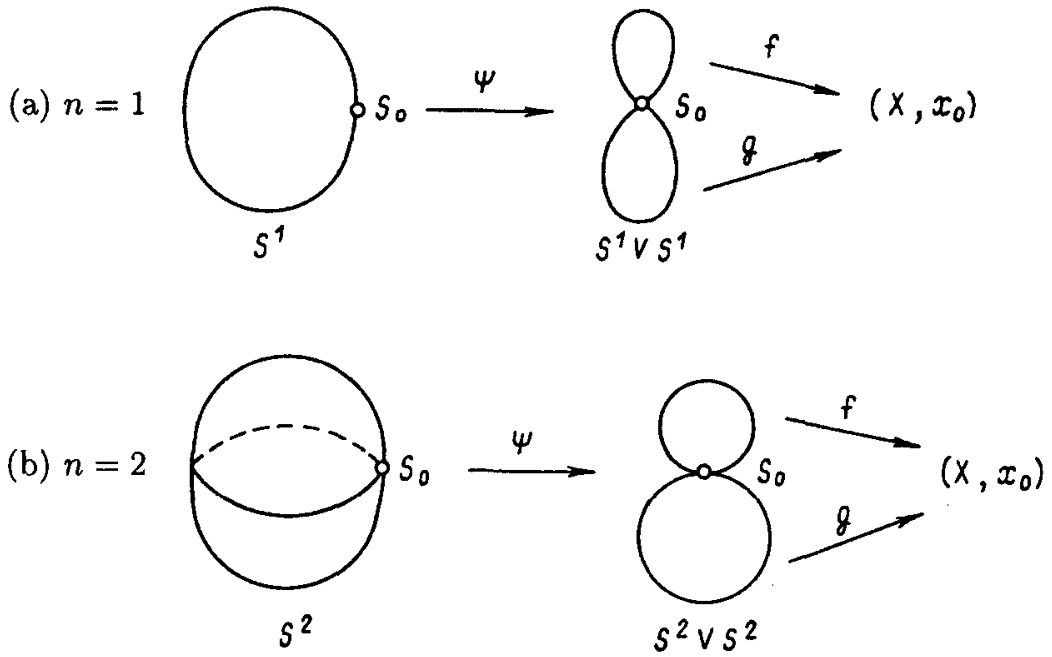
\includegraphics[width=0.66\textwidth]{figures/fig2_5.png}
  \figtitle{2.5}{$f+g=(f\vee g)\circ\psi$}
\end{figure}

我们还没有指定这个集合的元素（即同伦类）上如何做群运算。设 $f,g$ 是两个映射 $(S^n,s_0)\to(X,x_0)$。它们的\emph{和}定义为如下复合：先取把 $S^n$ 映到楔和 $S^n\vee S^n$ 的映射 $\psi$（它把 $S^n$ 的赤道收缩为赤道上的点 $s_0$），然后取楔和到空间 $(X,x_0)$ 的映射，它在楔和的第一个球面上与 $f$ 一致，在第二个球面上与 $g$ 一致（见图 2.5）。
% [原文 p.25]
推广到映射的同伦类上，这个和是良定义的，并给出 $\pi_n(X,x_0)$ 上的群运算（见图 2.6、图 2.7）。对 $n>1$，这个群运算是交换的；原因是 $n>1$ 时 $n$ 维球面可以在保持点 $s_0$ 不动的条件下连续旋转，从而交换它的上、下两个半球（见图 2.8）。因此对 $n>1$，$\pi_n(X,x_0)$ 上的群运算采用加法记号。

\begin{figure}[htbp]
  \centering
  \begin{minipage}{0.47\textwidth}
    \centering
    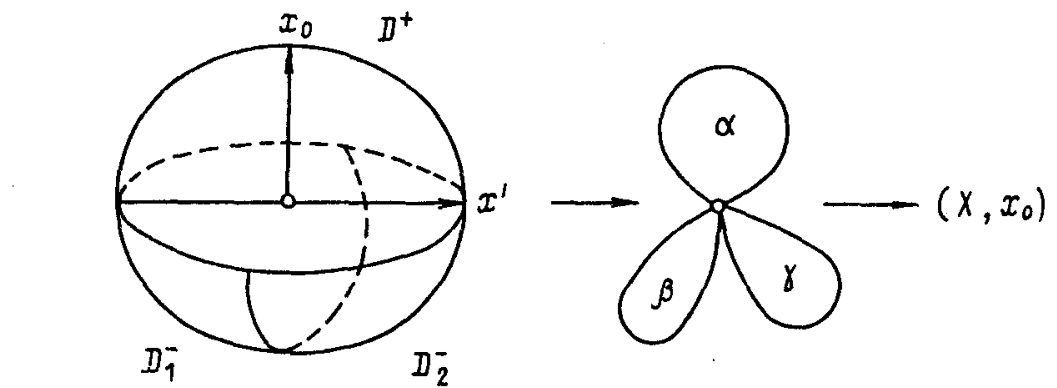
\includegraphics[width=\textwidth]{figures/fig2_6.png}
    \figtitle{2.6}{}
  \end{minipage}\hfill
  \begin{minipage}{0.47\textwidth}
    \centering
    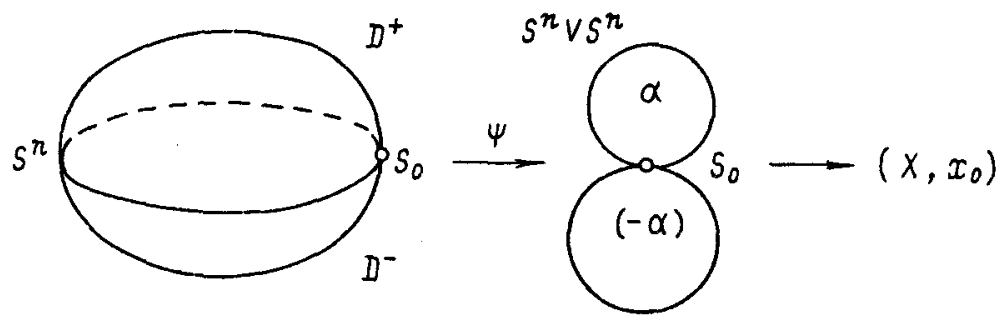
\includegraphics[width=0.92\textwidth]{figures/fig2_7.png}
    \figtitle{2.7}{}
  \end{minipage}
\end{figure}
\begin{figure}[htbp]
  \centering
  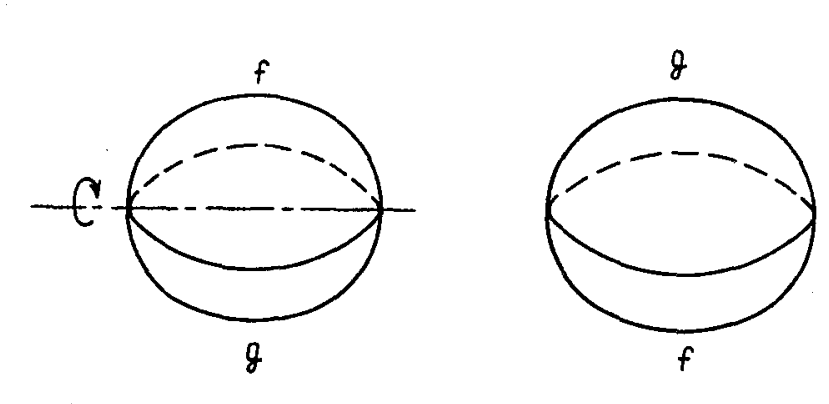
\includegraphics[width=0.56\textwidth]{figures/fig2_8.png}
  \figtitle{2.8}{}
\end{figure}
% [Tutor Note: 交换性的标准论证是 Eckmann--Hilton：$n>1$ 时 $\pi_n$ 上存在两个互相分配（即各自与对方的复合都同伦）的群运算，两个分配运算必然相同且交换。原书用「球面可以连续旋转」来述说这件事；关键正是旋转把两次「和」的次序调换过来，而 $n=1$ 时赤道上没有可旋转的空间。]

% [原文 p.26]
注意，$\pi_n(X,x_0)$ 的元素也可以实现为圆盘 $D^n$ 的映射 $f$ 的同伦类，只要把边界 $\partial D^n=S^{n-1}$ 映到点 $x_0$：
\[
  f:(D^n,S^{n-1})\to(X,x_0).
\]
$X$ 中任意一条道路 $\gamma(t)$，$1\le t\le 2$，只要它始于 $\gamma(1)=x_0$、终于 $\gamma(2)=x_1$，就给出柱面 $S^{n-1}\times I$ 到 $X$ 的映射
\[
  S^{n-1}\times I\to I\xrightarrow{\gamma}X,
\]
它只依赖于坐标 $t$。若把这个映射与任意映射 $f:(D^n,S^{n-1})\to(X,x_0)$ 并起来，就得到后一映射沿道路 $\gamma$ 的延拓：
\[
  (f,\gamma):\bigl(D^n\cup(S^{n-1}\times I),\,S^{n-1}\times\{2\}\bigr)\to(X,x_1).
\]
借助这一构造，我们得到不同基点的第 $n$ 个同伦群之间的自然同构（见图 2.9、图 2.10、图 2.11）：
\[
  \gamma_*^{(n)}:\pi_n(X,x_0)\to\pi_n(X,x_1).
\]

\begin{figure}[htbp]
  \centering
  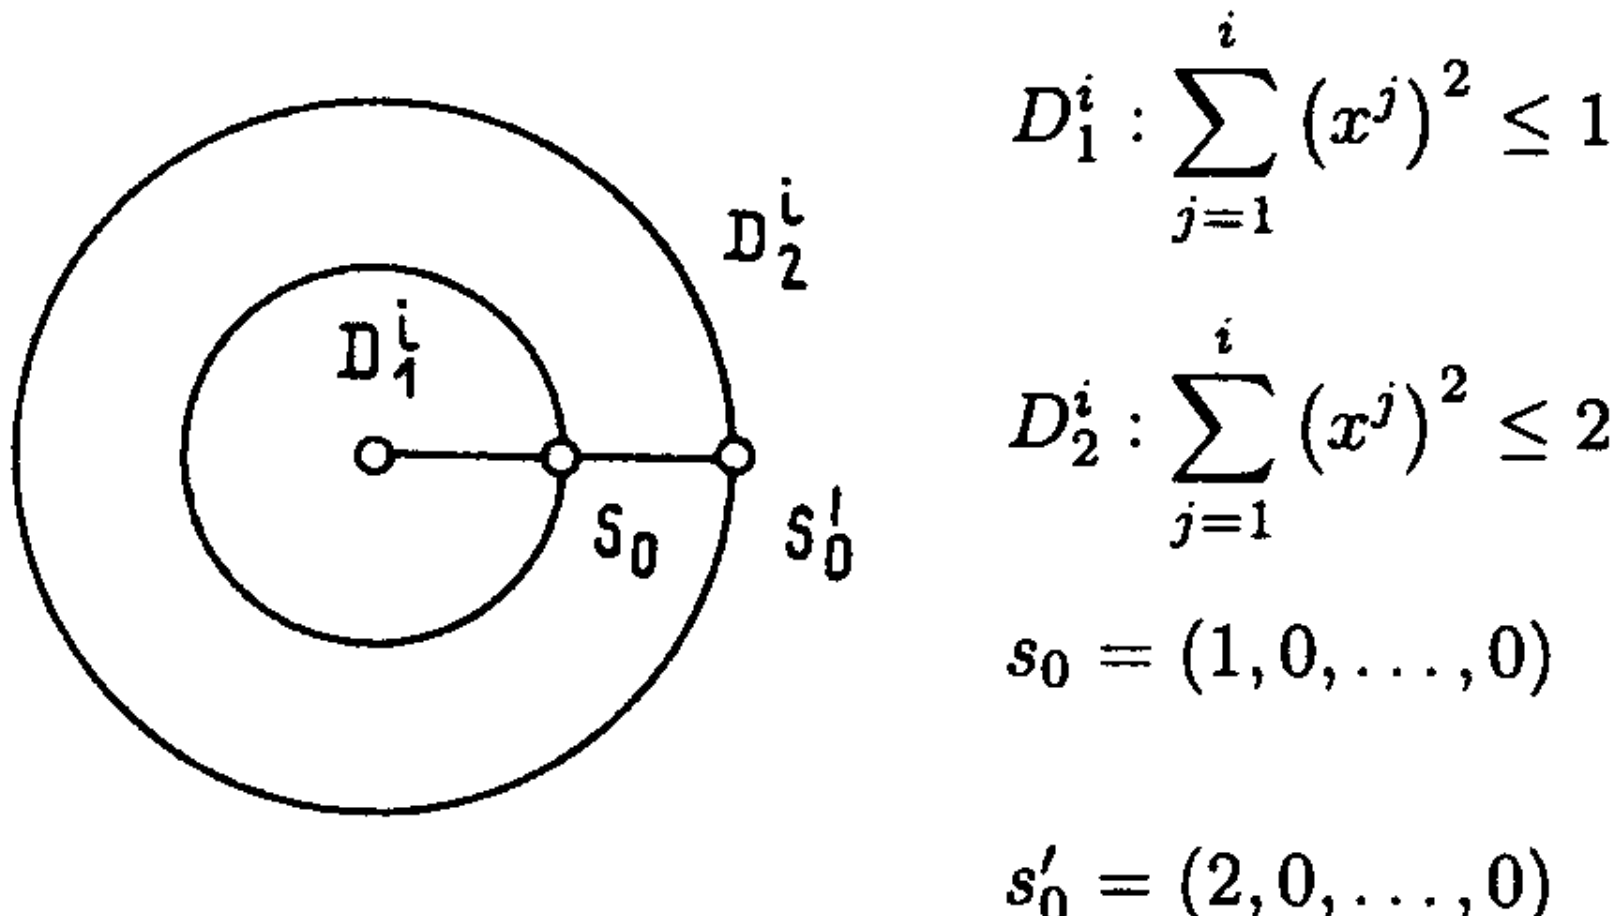
\includegraphics[width=0.62\textwidth]{figures/fig2_9.png}
  \figtitle{2.9}{}
\end{figure}
\begin{figure}[htbp]
  \centering
  \begin{minipage}{0.46\textwidth}
    \centering
    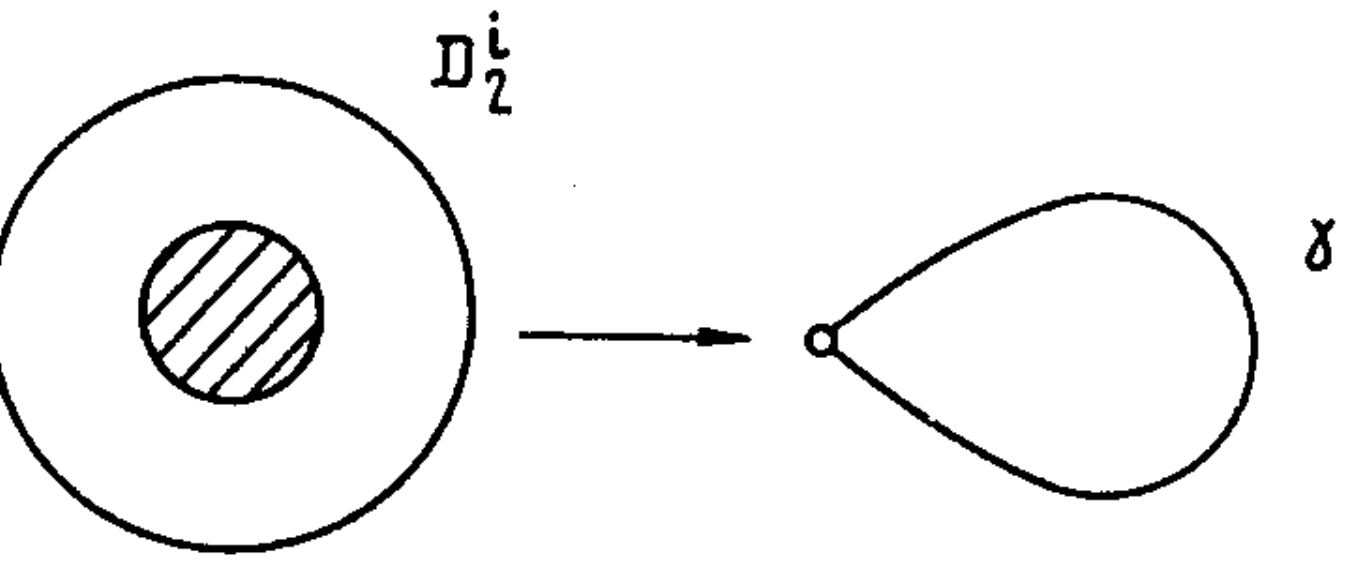
\includegraphics[width=\textwidth]{figures/fig2_10.png}
    \figtitle{2.10}{}
  \end{minipage}\hfill
  \begin{minipage}{0.46\textwidth}
    \centering
    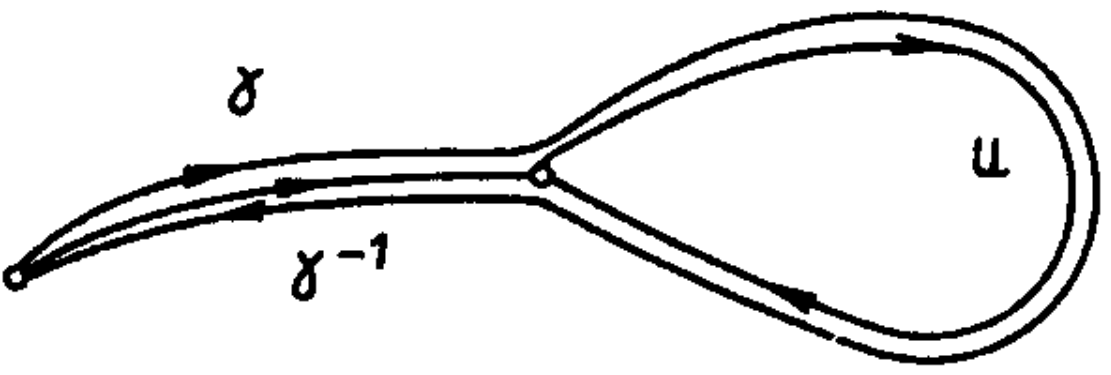
\includegraphics[width=\textwidth]{figures/fig2_11.png}
    \figtitle{2.11}{}
  \end{minipage}
\end{figure}

% [原文 p.27]
同构 $\gamma_*^{(n)}$ 只依赖于道路 $\gamma$ 在连接 $x_0$ 与 $x_1$ 的全部道路之集里的同伦类。当 $x_0=x_1$ 时，每个这样的同伦类都是以 $x_0$ 为基点的环路同伦类，从而是第一个同伦群 $\pi_1(X,x_0)$（即 $(X,x_0)$ 的\emph{基本群}）的元素。由此可知，基本群 $\pi_1(X,x_0)$ 自然地作为算子群作用在每个群 $\pi_n(X,x_0)$ 上。对 $n=1$，这个作用就是诱导 $\pi_1$ 内自同构的共轭作用（见图 2.12、图 2.13）：
\[
  \gamma_*^{(1)}(u)=\gamma\cdot u\cdot\gamma^{-1},\quad u\in\pi_1,\ \gamma\in\pi_1.
\]
\begin{figure}[htbp]
  \centering
  \begin{minipage}{0.40\textwidth}
    \centering
    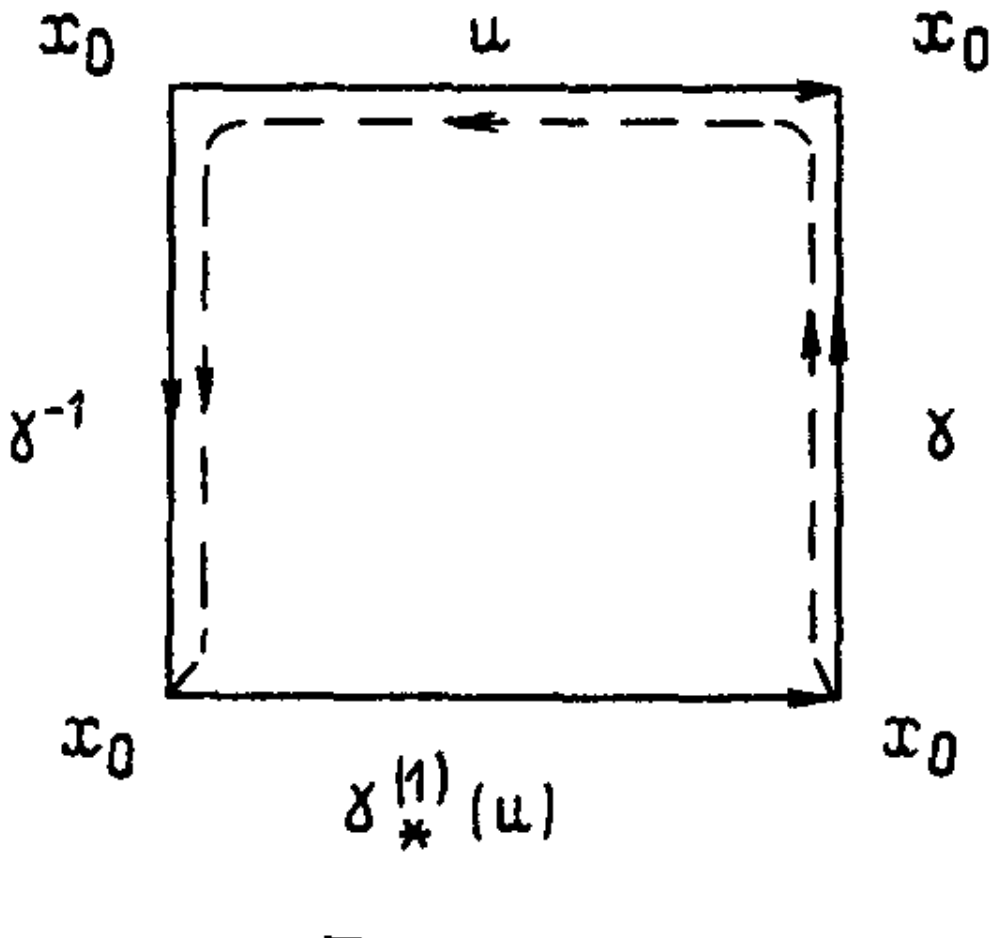
\includegraphics[width=\textwidth]{figures/fig2_12.png}
    \figtitle{2.12}{}
  \end{minipage}\hfill
  \begin{minipage}{0.52\textwidth}
    \centering
    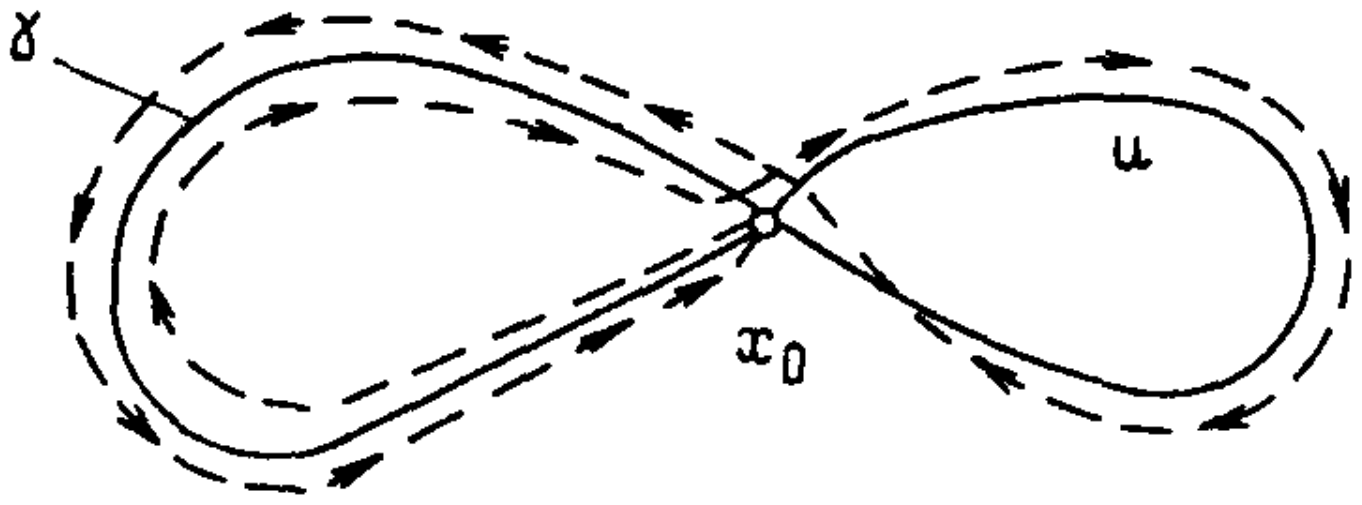
\includegraphics[width=\textwidth]{figures/fig2_13.png}
    \figtitle{2.13}{}
  \end{minipage}
\end{figure}

一类非常重要的拓扑空间是\emph{单连通的}空间，即基本群 $\pi_1(X,x_0)$ 平凡的空间。在这种情形下，由上面的讨论可知，同伦群 $\pi_n(X,x_0)$ 本质上不依赖于基点 $x_0$ 的选取（对道路连通的空间 $X$ 而言）；$\pi_n(X,x_0)$ 可以直接定义为映射 $S^n\to X$ 的自由同伦类之集，而不指定基点。在一般情形（连通但不必单连通的空间），映射 $S^n\to X$ 的自由同伦类（即不带点的同伦类）可以代数地确定为群 $\pi_n(X,x_0)$ 在 $\pi_1=\pi_1(X,x_0)$ 作用下的轨道。当 $n=1$ 时，这些正是群 $\pi_1$ 的共轭类。

由定义容易推出，两个空间之积的第 $n$ 个同伦群就是各因子空间的第 $n$ 个同伦群之直积：
\[
  \pi_n(X\times Y,x_0\times y_0)=\pi_n(X,x_0)\times\pi_n(Y,y_0).
\]
此外还有空间的 \emph{smash 积}（或称\emph{张量积}）：
\[
  X\wedge Y=X\times Y/(X\times y_0)\vee(x_0\times Y),
\]
其中 $X$、$Y$ 与 $X\wedge Y$ 的同伦群之间的关系由同伦群的\emph{双线性配对}给出：
% [原文 p.28]
\[
  \Phi:\pi_l(X)\otimes\pi_m(Y)\to\pi_{l+m}(X\wedge Y),
\]
其中 $\Phi$ 具有形式
\[
  \Phi=(f,g),\quad f:S^l\to X,\quad g:S^m\to Y,\quad S^{l+m}\cong S^l\wedge S^m.
\]
% [Tutor Note: 这个配对把「球面的乘积 $\cong$ smash 积」与 $\pi_l\otimes\pi_m$ 联系起来，是后文同调论中叉积（cross-product）的同伦版本；注意两个因子的基点必须与 $X\wedge Y$ 中的粘合点对应，且 $S^{l+m}\cong S^l\wedge S^m$ 用的是标准的「经线重排」同胚。]

对任意群 $\pi$，定义 $\pi$ 的\emph{整群环} $\Z[\pi]$：其元素是 $\pi$ 中元素、以整数为系数的有限形式线性组合：
\[
  a=\sum_{i=1}^N\lambda_i u_i,\quad \lambda_i\in\Z,\ u_i\in\pi.
\]
加法就是线性组合的通常加法，乘法定义如下：给定 $a=\sum\lambda_i u_i$、$b=\sum\mu_j v_j$，令
\begin{equation}
  a\cdot b=\Bigl(\sum\lambda_i u_i\Bigr)\cdot\Bigl(\sum\mu_j v_j\Bigr)
  =\sum_{i,j}\lambda_i\mu_j\,(u_i\cdot v_j). \tag{4.1}
\end{equation}
（整）群环还有一个等价定义，在分析学的语境中更常用：元素取为具有有限支撑的函数 $a:\pi\to\Z$（$u_i\mapsto\lambda_i$），按整值函数的通常方式相加，乘法按「卷积」如下给出：给定两个这样的函数 $a,b$，其积为
\begin{equation}
  a\cdot b(u)=\sum_{v\cdot w=u}a(v)b(w)=\sum_{v\in\pi}a(v)b(v^{-1}u). \tag{4.2}
\end{equation}
如前所述，这是同一个环 $\Z[\pi]$。把求和换成积分，这一概念可推广到连续（即拓扑）群的情形。
% [Tutor Note: (4.1) 中群 $\pi$ 不必交换，故 $\Sigma$ 里的次序、以及 $u_i\cdot v_j$ 的写法都不能随意调换；若 $\pi$ 非交换，$\Z[\pi]$ 是「斜」的——既有左模也有右模结构，二者一般不同。定义 4.2 之后的 $\Z[\pi]$-模结构默认取左模。]

对我们来说要点在于：用代数的语言说，每个同伦群 $\pi_n(X,x_0)$（$n>1$）都自然地是 $\Z[\pi]$-模，其中 $\pi=\pi_1(X,x_0)$；也就是说，它具有以 $\Z[\pi]$ 为「标量」环的线性空间的结构。

基本群 $\pi_1$ 由 Poincaré 引入。直到 1930 年代，高阶同伦群 $\pi_n$（$n>1$）才被定义（由 Hurewicz）。起初，这些群的 $\Z[\pi]$-模结构未被注意，而 $\pi_n$（$n>1$）的交换性造成了一种它们比 $\pi_1$ 形式上简单的假象。直到稍晚（自 Whitehead 于 1940 年代某时开始），它们的模结构才被使用——不过相当不系统。高阶同伦群的 $\Z[\pi]$-模结构被积极而系统地利用，是
自 1960 年代起、在非单连通流形理论的密集发展过程中才开始的。有趣的是，在同调论的某些特定问题里，模论式的考虑早在 1930 年代就已起过重要作用。
% [原文 p.29]

现在转向三元组 $(x_0\in A\subset X)$ 的范畴。

\begin{definition*}{4.2}
$n$ 维\emph{相对同伦群} $\pi_n(X,A,x_0)$（$n>1$）以映射
\[
  f:(D^n,S^{n-1},s_0)\to(X,A,x_0)
\]
的同伦类为元素，其中 $f(S^n)\subset A$，$f(s_0)=x_0$。群结构按与相应的绝对同伦群类似的方式定义在这个集合上（见图 2.14）。
\end{definition*}
% [Tutor Note: 原书 p.29 此条件印作 $f(S^n)\subset A$，但 $f$ 的定义域里球面部分是 $S^{n-1}$，故应为 $f(S^{n-1})\subset A$；正文照原书，读者按此修正理解即可，切勿据此把相对同伦群记成别的定义。]

可以证明，$n>2$ 时群 $\pi_n(X,A,x_0)$ 是交换的。这里起算子群作用的是群 $\pi_1(A,x_0)$，它作用在诸 $\pi_n(X,A,x_0)$（$n>2$）上，因此可以把这些群看作 $\Z[\pi]$-模，其中 $\pi=\pi_1(A,x_0)$。

\begin{figure}[htbp]
  \centering
  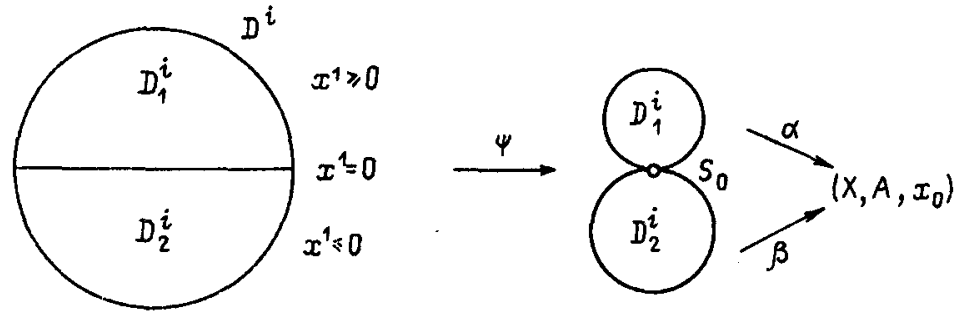
\includegraphics[width=0.62\textwidth]{figures/fig2_14.png}
  \figtitle{2.14}{}
\end{figure}

在「相对」框架下出现三个自然的同态：
\begin{align}
  j_*&:\pi_n(X,x_0)\to\pi_n(X,A,x_0),\notag\\
  \partial&:\pi_n(X,A,x_0)\to\pi_{n-1}(A,x_0),\tag{4.3}\\
  i_*&:\pi_n(A,x_0)\to\pi_n(X,x_0).\notag
\end{align}
同态 $j_*$ 的定义基于如下观察：映射 $f:(D^n,S^{n-1})\to(X,x_0)$ 可以看作三元组的映射 $g$：
\[
  f=g:(D^n,S^{n-1},s_0)\to(X,A,x_0),
\]
因为 $x_0\in A$。

同态 $\partial$ 的定义是：把映射 $f:(D^n,S^{n-1})\to(X,A,x_0)$ 限制到 $D^n$ 的边界 $\partial D^n=S^{n-1}$ 上：
% [原文 p.30]
\[
  g=f|_{S^{n-1}}:(S^{n-1},s_0)\to(A,x_0).
\]
「包含同态」$i_*$ 直接来自包含映射 $A\subset X$。
% [Tutor Note: 注意 $\partial$ 的构造在几何上就是「把 $S^{n-1}$ 上的映射当作 $n$ 维闭链的边界」这一步；它既是同伦正合列 (4.5) 的连接同态，也是第 3 章里相对同调列连接同态的同伦原型。$j_*$、$i_*$ 的记号方向容易记反：$i$ 是 $A\hookrightarrow X$，$j$ 是空间对 $(X,\varnothing)\hookrightarrow(X,A)$。]

几乎显然的是，任意两个「相邻」同态 $i_*,j_*,\partial$ 的复合都给出零同态：
\[
  j_*\circ i_*=0,\qquad \partial\circ j_*=0,\qquad i_*\circ\partial=0,
\]
由此推得
\[
  \Image i_*\subset\Ker j_*,\qquad \Image j_*\subset\Ker\partial,\qquad \Image\partial\subset\Ker i_*.
\]
（稍作计算可知）这些子群包含关系实际上都是等式（称为「正合性条件」）：
\begin{equation}
  \Image i_*=\Ker j_*,\qquad \Image j_*=\Ker\partial,\qquad \Image\partial=\Ker i_*. \tag{4.4}
\end{equation}
这通常表述为：下列群与同态的序列是「正合的」：
\begin{equation}
  \cdots\to\pi_n(A,x_0)\xrightarrow{i_*}\pi_n(X,x_0)\xrightarrow{j_*}\pi_n(X,A,x_0)
  \xrightarrow{\partial}\pi_{n-1}(A,x_0)\to\cdots \tag{4.5}
\end{equation}
这个序列称为空间对 $(X,A)$ 的\emph{正合同伦序列}。
% [Tutor Note: 正合列 (4.5) 对任意空间对 $(X,A,x_0)$ 都成立：$n\ge2$ 时三个映射都是群同态，$n=1$ 时 $\pi_1(X,A,x_0)$ 只是带基点的集合、正合性按集合理解。真正需要额外假设的不是这条列，而是后文 (4.6)：只有 $F_0$ 是纤维化 $p:X\to Y$ 的纤维时，相对群 $\pi_n(X,F_0,x_0)$ 才能与 $\pi_n(Y,y_0)$ 等同，于是长列化为「纤维—全空间—底空间」的正合列而可算；对一般子空间 $A$，(4.5) 虽然正合，却无法把相对群换成已知的绝对群。]

同伦群的构造——一方面是绝对同伦群 $\pi_n(X,x_0)$，另一方面是相对同伦群 $\pi_n(X,A,x_0)$——可以看作从带点拓扑空间范畴（或三元组范畴，视情形而定）到（交换）群范畴的\emph{共变函子}。这无非是说，带点空间 $(X,x_0)$（或三元组 $(X,A,x_0)$）的映射
\[
  f:X\to Y,\quad x_0\to y_0,\quad (A\to B)
\]
给出相应同伦群之间的同态
\[
  f_*:\pi_n(X,x_0)\to\pi_n(Y,y_0),
\]
\[
  f_*:\pi_n(X,A,x_0)\to\pi_n(Y,B,y_0).
\]
这些同态本质上是这样得到的：对每个代表 $\pi_n(X,x_0)$ 中元素的映射 $g:(D^n,S^{n-1})\to(X,x_0)$，联系以映射
\[
  f\circ g:(D^n,S^{n-1})\to(Y,y_0),
\]
三元组的情形类似。在上述几例中我们有
\[
  i:A\to X,\quad i(x_0)=x_0,
\]
\[
  i_*:\pi_n(A,x_0)\to\pi_n(X,x_0),
\]
（即包含同态），以及
\[
  j:\begin{cases}
    X\to X\\
    x_0\to A\\
    x_0\to x_0
  \end{cases},
\]
% [原文 p.31]
\[
  j_*:\pi_n(X,x_0,x_0)=\pi_n(X,x_0)\to\pi_n(X,A,x_0).
\]
% [Tutor Note: 上面的 $j$ 是三行排法，按约定读作「三元组的映射 $(X,x_0,x_0)\to(X,A,x_0)$」：第一行说空间 $X$ 映到 $X$，第二行说作为子空间的 $\{x_0\}$ 映入 $A$，第三行说基点 $x_0$ 映到 $x_0$。于是 $\pi_n(X,x_0,x_0)$ 就化归为绝对同伦群 $\pi_n(X,x_0)$。]

上面这组同伦群（以及同调群）的初等性质——特别是它们的函子性与空间对 $(X,A)$ 的正合列——经过进一步实质性的发展，导出了拓扑学的整套精细代数工具，下文将会看到。

有一种极为重要的情形，与计算同伦群的代数方法密切相关：其中相对同伦群归结为绝对同伦群。考虑任意纤维化 $p:X\to Y$，它具有覆叠同伦性质（照例是对 $t=0$ 处任意给定的初始条件而言）。设 $y_0\in Y$，$x_0\in p^{-1}(y_0)=F_0$。一个重要（尽管并不特别困难）的定理断言存在同构
\begin{equation}
  \pi_n(X,F_0,x_0)\cong\pi_n(Y,y_0). \tag{4.6}
\end{equation}
这用投影同态 $p_*$ 来建立（$p_*$ 来自把纤维 $F_0$ 映到点 $y_0$ 的投影 $p:X\to Y$）。从覆叠同伦性质出发，可以如下直观地看出这个同构。每个代表 $\pi_n(Y,y_0)$ 中元素的映射 $f:D^n\to Y$，都可以提升到 $X$，理由是圆盘 $D^n$ 可缩到其边界 $S^{n-1}$ 上的点 $s_0$（见图 2.15）。把该映射提升到 $X$，得到覆叠映射 $D^n\to X$，它把边界 $S^{n-1}$ 不一定映成一点，而是映入 $y_0$ 上方的纤维 $F_0$。一个直接的论证现在给出所要的同构 (4.6)。
\begin{figure}[htbp]
  \centering
  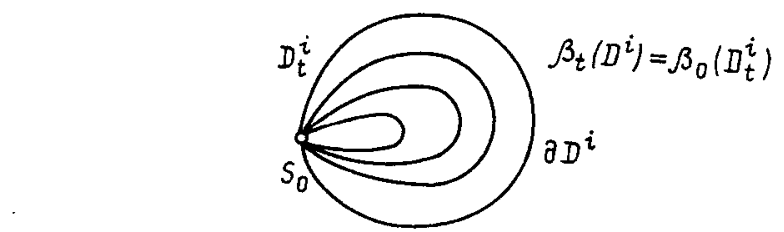
\includegraphics[width=0.58\textwidth]{figures/fig2_15.png}
  \figtitle{2.15}{}
\end{figure}
% [Tutor Note: 这一步「先提升、再看边界落进纤维」正是纤维化正合列 $\pi_n(F_0)\to\pi_n(X)\to\pi_n(Y)\xrightarrow{\partial}\pi_{n-1}(F_0)$ 的几何来源：$f:D^n\to Y$ 提升后边界落在 $F_0$ 中，于是给出 $S^{n-1}\to F_0$ 的映射，那就是 $\partial$。]

这个同构最终来自覆叠同伦性质；作为它的推论，人们得到纤维化的如下正合列（而不是空间对 $(X,F_0)$ 的正合列）：
% CHUNK ch02b DONE
